% ===============================================================
% Entrega 4: Integracao do Codigo e Boilerplate Vulkan
% Incluido no main.tex com % ===============================================================
% Entrega 4: Integracao do Codigo e Boilerplate Vulkan
% Incluido no main.tex com % ===============================================================
% Entrega 4: Integracao do Codigo e Boilerplate Vulkan
% Incluido no main.tex com % ===============================================================
% Entrega 4: Integracao do Codigo e Boilerplate Vulkan
% Incluido no main.tex com \input{entrega4}
% ===============================================================

\section{Integração do Código e Boilerplate Vulkan}
\label{sec:boilerplate}
\sloppy

Esta seção documenta a quarta entrega do trabalho, cujo objetivo é a construção da infraestrutura básica (\textit{boilerplate}) da aplicação gráfica em C++20 utilizando a API Vulkan, além da integração e validação dos \textit{shaders} desenvolvidos na Entrega 3 (Seção~\ref{sec:pseudocodigo}).

A aplicação desenvolvida abre uma janela interativa, inicializa as estruturas fundamentais do Vulkan, seleciona a GPU do sistema, configura a \textit{swapchain}, aloca os \textit{command buffers}, gerencia primitivas explícitas de sincronização (semáforos e \textit{fences}) e executa o ciclo de renderização na tela. Além disso, todos os oito \textit{shaders} em SPIR-V são carregados em módulos Vulkan (\texttt{VkShaderModule}) e utilizados pelo pipeline gráfico.

\subsection{Organização Modular do Projeto}
Em conformidade com os princípios da responsabilidade única (SOLID) e do código limpo (\textit{clean code}), o projeto foi estruturado em módulos independentes na pasta \texttt{src/}:

\begin{itemize}
    \setlength{\itemsep}{0pt}
    \item \textbf{\texttt{Janela} (\texttt{Janela.hpp/cpp}):} Encapsula a biblioteca GLFW, gerenciando a criação da janela sem contexto OpenGL, redimensionamentos e a criação da superfície \texttt{VkSurfaceKHR}.
    \item \textbf{\texttt{InstanciaVulkan} (\texttt{DispositivoVulkan.hpp/cpp}):} Configura a instância global da API (\texttt{VkInstance}), consulta extensões necessárias e ativa as camadas de validação (\texttt{VK\_LAYER\_KHRONOS\_validation}) com mensagens de depuração (\texttt{VkDebugUtilsMessengerEXT}).
    \item \textbf{\texttt{DispositivoVulkan} (\texttt{DispositivoVulkan.hpp/cpp}):} Identifica as GPUs físicas disponíveis, selecionando preferencialmente dispositivos dedicados (\textit{Discrete GPU}), consulta as famílias de filas com suporte a comandos gráficos e de apresentação, e cria o dispositivo lógico (\texttt{VkDevice}).
    \item \textbf{\texttt{GerenciadorSwapchain} (\texttt{GerenciadorSwapchain.hpp/cpp}):} Negocia com a superfície o melhor formato de cores (preferencialmente \texttt{VK\_FORMAT\_B8G8R8A8\_SRGB}), o modo de apresentação (\textit{Mailbox} para \textit{triple buffering} ou \textit{FIFO}) e a resolução real dos \textit{framebuffers}, instanciando as respectivas \texttt{VkImageView}s. Trata também a recriação automática da cadeia de troca quando a janela é redimensionada.
    \item \textbf{\texttt{CarregadorShader} (\texttt{CarregadorShader.hpp/cpp}):} Lê os arquivos binários compilados em SPIR-V (\texttt{.spv}) do disco e instancia os respectivos módulos Vulkan (\texttt{VkShaderModule}), gerenciando sua validação e destruição controlada.
    \item \textbf{\texttt{PipelineGrafico} (\texttt{PipelineGrafico.hpp/cpp}):} Define o \textit{Render Pass} com transições de layout, cria os \textit{Framebuffers} vinculados às imagens da \textit{swapchain} e monta o pipeline gráfico de rasterização com estágios programáveis e estados dinâmicos (\textit{viewport} e \textit{scissor}).
    \item \textbf{\texttt{AplicacaoVulkan} (\texttt{AplicacaoVulkan.hpp/cpp}):} Orquestra o ciclo de vida completo: cria o \textit{Command Pool}, aloca os \textit{Command Buffers}, inicializa semáforos e cercas (\textit{fences}) para sincronização de múltiplos quadros em voo (\textit{frames in flight}), grava os comandos de desenho e controla o laço principal (\textit{main loop}).
\end{itemize}

\subsection{Compilação dos Shaders para SPIR-V}
Os \textit{shaders} desenvolvidos em sintaxe GLSL na Entrega 3 foram compilados para o formato binário padrão do Vulkan (SPIR-V) por meio do compilador oficial \texttt{glslc}, componente do Vulkan SDK.

Foi criado o script automatizado \texttt{compilar\_shaders.sh}, que percorre todos os arquivos \texttt{.vert} e \texttt{.frag} da pasta \texttt{shaders/} e gera as saídas equivalentes em \texttt{shaders/spv/}. Além disso, o sistema de build \texttt{CMakeLists.txt} integra esse alvo (\texttt{compilar\_shaders}) antes da compilação do executável principal, garantindo que qualquer alteração nos \textit{shaders} seja automaticamente refletida nos binários SPIR-V.

\begin{table}[H]
    \centering
    \caption{\textit{Shaders} SPIR-V integrados e carregados na aplicação Vulkan.}
    \label{tab:shaders_spv}
    \vspace{4pt}
    \small
    \begin{tabular}{l l l p{6.5cm}}
        \toprule
        \textbf{Arquivo Fonte} & \textbf{Binário SPIR-V} & \textbf{Estágio} & \textbf{Papel na Técnica de Bloom} \\
        \midrule
        \texttt{scene.vert} & \texttt{scene.vert.spv} & \textit{Vertex} & Transformação de geometria 3D da cena \\
        \texttt{scene.frag} & \texttt{scene.frag.spv} & \textit{Fragment} & Iluminação direta e saída HDR sem corte \\
        \texttt{fullscreen.vert} & \texttt{fullscreen.vert.spv} & \textit{Vertex} & Geração procedural do triângulo de tela cheia \\
        \texttt{bright.frag} & \texttt{bright.frag.spv} & \textit{Fragment} & Isolamento de altas luzes (\textit{bright pass}) \\
        \texttt{downsample.frag} & \texttt{downsample.frag.spv} & \textit{Fragment} & Redução piramidal e filtro de 13 amostras \\
        \texttt{upsample.frag} & \texttt{upsample.frag.spv} & \textit{Fragment} & Expansão piramidal e filtro tenda $3\times3$ \\
        \texttt{composite.frag} & \texttt{composite.frag.spv} & \textit{Fragment} & Composição da cena com \textit{Bloom} e \textit{Tone Mapping} \\
        \texttt{teste.frag} & \texttt{teste.frag.spv} & \textit{Fragment} & Fragmento de teste visual com gradiente e núcleo luminoso \\
        \bottomrule
    \end{tabular}
\end{table}

\subsection{Ferramentas, Bibliotecas e Ambiente de Execução}
A infraestrutura foi construída e validada no seguinte ambiente técnico:
\begin{itemize}
    \setlength{\itemsep}{0pt}
    \item \textbf{Linguagem e Padrão:} C++20 (ISO/IEC 14882:2020), utilizando recursos como \texttt{std::optional}, ponteiros inteligentes (\texttt{std::unique\_ptr}) e verificação rigorosa de tipos.
    \item \textbf{Compilador:} GNU Compiler Collection (\texttt{g++} 16.2.1 / \texttt{gcc}) com suporte a flags de otimização e checagem estrita de avisos (\texttt{-Wall -Wextra -Wpedantic}).
    \item \textbf{Sistema de Build:} CMake versão 3.20 ou superior.
    \item \textbf{Vulkan SDK / Header:} Vulkan API versão 1.3 / 1.4 (especificação 1.4.364), biblioteca carregadora \texttt{libvulkan.so.1}.
    \item \textbf{Compilador de Shaders:} \texttt{glslc} (Vulkan Shader Compiler via Google Shaderc).
    \item \textbf{Bibliotecas Auxiliares:} GLFW 3.3 (gerenciamento de janelas e contexto de superfície do sistema operacional) e GLM (álgebra linear e estruturas matriciais/vetoriais).
    \item \textbf{GPU de Execução:} NVIDIA GeForce RTX 3080 (driver proprietário versão 615.71, suporte nativo à API Vulkan 1.4).
\end{itemize}

\subsection{Instruções de Compilação e Execução}

Para compilar e executar o projeto no Linux a partir do terminal:

\begin{enumerate}
    \item \textbf{Compilação dos Shaders (opcional, já acoplada ao CMake):}
    \begin{verbatim}
    ./compilar_shaders.sh
    \end{verbatim}
    \item \textbf{Geração dos arquivos de build com CMake:}
    \begin{verbatim}
    cmake -B build
    \end{verbatim}
    \item \textbf{Compilação do executável:}
    \begin{verbatim}
    cmake --build build
    \end{verbatim}
    \item \textbf{Execução da aplicação:}
    \begin{verbatim}
    ./build/BloomVulkan
    \end{verbatim}
    Para testes automatizados sem intervenção de usuário, a aplicação aceita o parâmetro \texttt{--quadros N} (ou \texttt{--teste}), que renderiza $N$ quadros, exporta a comprovação visual e finaliza de forma limpa.
\end{enumerate}

\subsection{Comprovação Visual e Funcionamento}
Ao executar a aplicação, o Vulkan inicializa a superfície de apresentação na janela criada via GLFW e associa o pipeline gráfico aos módulos SPIR-V \texttt{fullscreen.vert.spv} e \texttt{teste.frag.spv}. 

O \texttt{fullscreen.vert} gera dinamicamente as coordenadas do triângulo de tela cheia sem necessidade de \textit{vertex buffer} físico, e o \textit{fragment shader} interpola as coordenadas UV de tela cheia, desenhando um gradiente de luminância e um núcleo emissivo incandescente central. A Figura~\ref{fig:captura_execucao} ilustra a captura de tela direta gerada na renderização da GPU.

\begin{figure}[H]
    \centering
    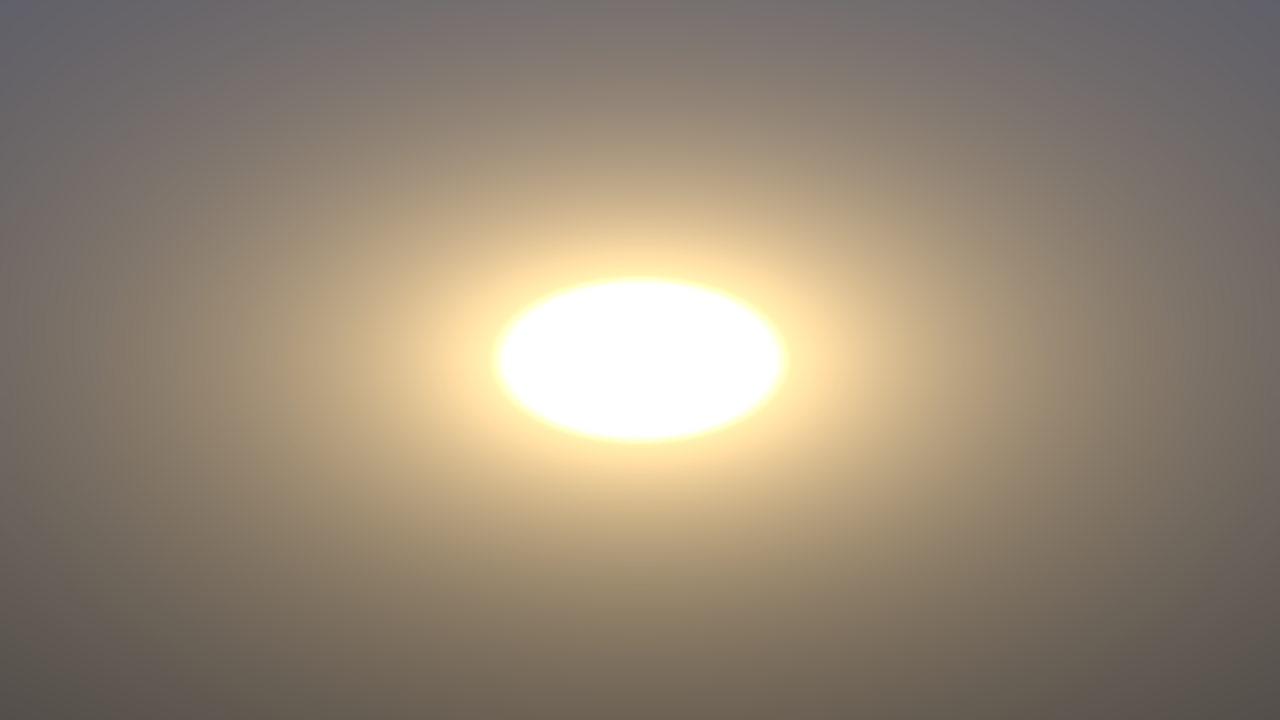
\includegraphics[width=0.82\textwidth]{captura_execucao.png}
    \caption{Captura de tela obtida diretamente do \textit{framebuffer} durante a execução do programa em Vulkan. Demonstra a operação integrada da janela GLFW, \textit{swapchain}, alocação de comandos na GPU e execução dos \textit{shaders} SPIR-V via pipeline gráfico.}
    \label{fig:captura_execucao}
\end{figure}

\subsection{Funcionalidades Concluídas e Próximos Passos}

\textbf{Funcionalidades Implementadas e Validadas nesta Etapa:}
\begin{itemize}
    \setlength{\itemsep}{0pt}
    \item Inicialização completa da instância Vulkan e integração das camadas de validação;
    \item Seleção automática de GPU discreta de alto desempenho e criação do dispositivo lógico;
    \item Identificação e separação das filas gráficas e de apresentação;
    \item Configuração dinâmica e segura da \textit{swapchain} e instanciação das \textit{Image Views};
    \item Criação de \textit{Render Pass}, \textit{Pipeline Layout}, \textit{Framebuffers} e \textit{Pipeline Gráfico};
    \item Alocação de \textit{Command Pool} e múltiplos \textit{Command Buffers};
    \item Sincronização explícita via semáforos de aquisição/renderização e \textit{fences} de CPU-GPU;
    \item Laço principal de aquisição, gravação de comandos, submissão gráfica e apresentação na tela;
    \item Compilação e carga em memória de todos os oito \textit{shaders} SPIR-V projetados;
    \item Desalocação rigorosa e ordenada de todos os recursos da GPU no encerramento da aplicação.
\end{itemize}

\textbf{Funcionalidades para as Próximas Entregas (Técnica de Bloom Completa):}
Nas próximas etapas, o pipeline base construído aqui será expandido para materializar o fluxo completo de onze passes projetado na Entrega 2:
\begin{enumerate}
    \setlength{\itemsep}{0pt}
    \item Alocação dos anexos intermediários fora de tela (\textit{offscreen}) em ponto flutuante de 16 bits (\texttt{VK\_FORMAT\_R16G16B16A16\_SFLOAT}) para a imagem \texttt{sceneHDR};
    \item Criação da textura piramidal de \textit{Bloom} (\texttt{bloomMip[0]} a \texttt{bloomMip[4]});
    \item Configuração dos \textit{Descriptor Sets} e \textit{Uniform Buffers} (\texttt{BloomParams} e \texttt{CameraUBO});
    \item Encadeamento dos passes de \textit{downsample} e \textit{upsample} com mistura aditiva (\textit{additive blending});
    \item Inserção das barreiras de memória explícitas (\texttt{VkImageMemoryBarrier}) entre as etapas de escrita e leitura de texturas.
\end{enumerate}
\fussy

% ===============================================================

\section{Integração do Código e Boilerplate Vulkan}
\label{sec:boilerplate}
\sloppy

Esta seção documenta a quarta entrega do trabalho, cujo objetivo é a construção da infraestrutura básica (\textit{boilerplate}) da aplicação gráfica em C++20 utilizando a API Vulkan, além da integração e validação dos \textit{shaders} desenvolvidos na Entrega 3 (Seção~\ref{sec:pseudocodigo}).

A aplicação desenvolvida abre uma janela interativa, inicializa as estruturas fundamentais do Vulkan, seleciona a GPU do sistema, configura a \textit{swapchain}, aloca os \textit{command buffers}, gerencia primitivas explícitas de sincronização (semáforos e \textit{fences}) e executa o ciclo de renderização na tela. Além disso, todos os oito \textit{shaders} em SPIR-V são carregados em módulos Vulkan (\texttt{VkShaderModule}) e utilizados pelo pipeline gráfico.

\subsection{Organização Modular do Projeto}
Em conformidade com os princípios da responsabilidade única (SOLID) e do código limpo (\textit{clean code}), o projeto foi estruturado em módulos independentes na pasta \texttt{src/}:

\begin{itemize}
    \setlength{\itemsep}{0pt}
    \item \textbf{\texttt{Janela} (\texttt{Janela.hpp/cpp}):} Encapsula a biblioteca GLFW, gerenciando a criação da janela sem contexto OpenGL, redimensionamentos e a criação da superfície \texttt{VkSurfaceKHR}.
    \item \textbf{\texttt{InstanciaVulkan} (\texttt{DispositivoVulkan.hpp/cpp}):} Configura a instância global da API (\texttt{VkInstance}), consulta extensões necessárias e ativa as camadas de validação (\texttt{VK\_LAYER\_KHRONOS\_validation}) com mensagens de depuração (\texttt{VkDebugUtilsMessengerEXT}).
    \item \textbf{\texttt{DispositivoVulkan} (\texttt{DispositivoVulkan.hpp/cpp}):} Identifica as GPUs físicas disponíveis, selecionando preferencialmente dispositivos dedicados (\textit{Discrete GPU}), consulta as famílias de filas com suporte a comandos gráficos e de apresentação, e cria o dispositivo lógico (\texttt{VkDevice}).
    \item \textbf{\texttt{GerenciadorSwapchain} (\texttt{GerenciadorSwapchain.hpp/cpp}):} Negocia com a superfície o melhor formato de cores (preferencialmente \texttt{VK\_FORMAT\_B8G8R8A8\_SRGB}), o modo de apresentação (\textit{Mailbox} para \textit{triple buffering} ou \textit{FIFO}) e a resolução real dos \textit{framebuffers}, instanciando as respectivas \texttt{VkImageView}s. Trata também a recriação automática da cadeia de troca quando a janela é redimensionada.
    \item \textbf{\texttt{CarregadorShader} (\texttt{CarregadorShader.hpp/cpp}):} Lê os arquivos binários compilados em SPIR-V (\texttt{.spv}) do disco e instancia os respectivos módulos Vulkan (\texttt{VkShaderModule}), gerenciando sua validação e destruição controlada.
    \item \textbf{\texttt{PipelineGrafico} (\texttt{PipelineGrafico.hpp/cpp}):} Define o \textit{Render Pass} com transições de layout, cria os \textit{Framebuffers} vinculados às imagens da \textit{swapchain} e monta o pipeline gráfico de rasterização com estágios programáveis e estados dinâmicos (\textit{viewport} e \textit{scissor}).
    \item \textbf{\texttt{AplicacaoVulkan} (\texttt{AplicacaoVulkan.hpp/cpp}):} Orquestra o ciclo de vida completo: cria o \textit{Command Pool}, aloca os \textit{Command Buffers}, inicializa semáforos e cercas (\textit{fences}) para sincronização de múltiplos quadros em voo (\textit{frames in flight}), grava os comandos de desenho e controla o laço principal (\textit{main loop}).
\end{itemize}

\subsection{Compilação dos Shaders para SPIR-V}
Os \textit{shaders} desenvolvidos em sintaxe GLSL na Entrega 3 foram compilados para o formato binário padrão do Vulkan (SPIR-V) por meio do compilador oficial \texttt{glslc}, componente do Vulkan SDK.

Foi criado o script automatizado \texttt{compilar\_shaders.sh}, que percorre todos os arquivos \texttt{.vert} e \texttt{.frag} da pasta \texttt{shaders/} e gera as saídas equivalentes em \texttt{shaders/spv/}. Além disso, o sistema de build \texttt{CMakeLists.txt} integra esse alvo (\texttt{compilar\_shaders}) antes da compilação do executável principal, garantindo que qualquer alteração nos \textit{shaders} seja automaticamente refletida nos binários SPIR-V.

\begin{table}[H]
    \centering
    \caption{\textit{Shaders} SPIR-V integrados e carregados na aplicação Vulkan.}
    \label{tab:shaders_spv}
    \vspace{4pt}
    \small
    \begin{tabular}{l l l p{6.5cm}}
        \toprule
        \textbf{Arquivo Fonte} & \textbf{Binário SPIR-V} & \textbf{Estágio} & \textbf{Papel na Técnica de Bloom} \\
        \midrule
        \texttt{scene.vert} & \texttt{scene.vert.spv} & \textit{Vertex} & Transformação de geometria 3D da cena \\
        \texttt{scene.frag} & \texttt{scene.frag.spv} & \textit{Fragment} & Iluminação direta e saída HDR sem corte \\
        \texttt{fullscreen.vert} & \texttt{fullscreen.vert.spv} & \textit{Vertex} & Geração procedural do triângulo de tela cheia \\
        \texttt{bright.frag} & \texttt{bright.frag.spv} & \textit{Fragment} & Isolamento de altas luzes (\textit{bright pass}) \\
        \texttt{downsample.frag} & \texttt{downsample.frag.spv} & \textit{Fragment} & Redução piramidal e filtro de 13 amostras \\
        \texttt{upsample.frag} & \texttt{upsample.frag.spv} & \textit{Fragment} & Expansão piramidal e filtro tenda $3\times3$ \\
        \texttt{composite.frag} & \texttt{composite.frag.spv} & \textit{Fragment} & Composição da cena com \textit{Bloom} e \textit{Tone Mapping} \\
        \texttt{teste.frag} & \texttt{teste.frag.spv} & \textit{Fragment} & Fragmento de teste visual com gradiente e núcleo luminoso \\
        \bottomrule
    \end{tabular}
\end{table}

\subsection{Ferramentas, Bibliotecas e Ambiente de Execução}
A infraestrutura foi construída e validada no seguinte ambiente técnico:
\begin{itemize}
    \setlength{\itemsep}{0pt}
    \item \textbf{Linguagem e Padrão:} C++20 (ISO/IEC 14882:2020), utilizando recursos como \texttt{std::optional}, ponteiros inteligentes (\texttt{std::unique\_ptr}) e verificação rigorosa de tipos.
    \item \textbf{Compilador:} GNU Compiler Collection (\texttt{g++} 16.2.1 / \texttt{gcc}) com suporte a flags de otimização e checagem estrita de avisos (\texttt{-Wall -Wextra -Wpedantic}).
    \item \textbf{Sistema de Build:} CMake versão 3.20 ou superior.
    \item \textbf{Vulkan SDK / Header:} Vulkan API versão 1.3 / 1.4 (especificação 1.4.364), biblioteca carregadora \texttt{libvulkan.so.1}.
    \item \textbf{Compilador de Shaders:} \texttt{glslc} (Vulkan Shader Compiler via Google Shaderc).
    \item \textbf{Bibliotecas Auxiliares:} GLFW 3.3 (gerenciamento de janelas e contexto de superfície do sistema operacional) e GLM (álgebra linear e estruturas matriciais/vetoriais).
    \item \textbf{GPU de Execução:} NVIDIA GeForce RTX 3080 (driver proprietário versão 615.71, suporte nativo à API Vulkan 1.4).
\end{itemize}

\subsection{Instruções de Compilação e Execução}

Para compilar e executar o projeto no Linux a partir do terminal:

\begin{enumerate}
    \item \textbf{Compilação dos Shaders (opcional, já acoplada ao CMake):}
    \begin{verbatim}
    ./compilar_shaders.sh
    \end{verbatim}
    \item \textbf{Geração dos arquivos de build com CMake:}
    \begin{verbatim}
    cmake -B build
    \end{verbatim}
    \item \textbf{Compilação do executável:}
    \begin{verbatim}
    cmake --build build
    \end{verbatim}
    \item \textbf{Execução da aplicação:}
    \begin{verbatim}
    ./build/BloomVulkan
    \end{verbatim}
    Para testes automatizados sem intervenção de usuário, a aplicação aceita o parâmetro \texttt{--quadros N} (ou \texttt{--teste}), que renderiza $N$ quadros, exporta a comprovação visual e finaliza de forma limpa.
\end{enumerate}

\subsection{Comprovação Visual e Funcionamento}
Ao executar a aplicação, o Vulkan inicializa a superfície de apresentação na janela criada via GLFW e associa o pipeline gráfico aos módulos SPIR-V \texttt{fullscreen.vert.spv} e \texttt{teste.frag.spv}. 

O \texttt{fullscreen.vert} gera dinamicamente as coordenadas do triângulo de tela cheia sem necessidade de \textit{vertex buffer} físico, e o \textit{fragment shader} interpola as coordenadas UV de tela cheia, desenhando um gradiente de luminância e um núcleo emissivo incandescente central. A Figura~\ref{fig:captura_execucao} ilustra a captura de tela direta gerada na renderização da GPU.

\begin{figure}[H]
    \centering
    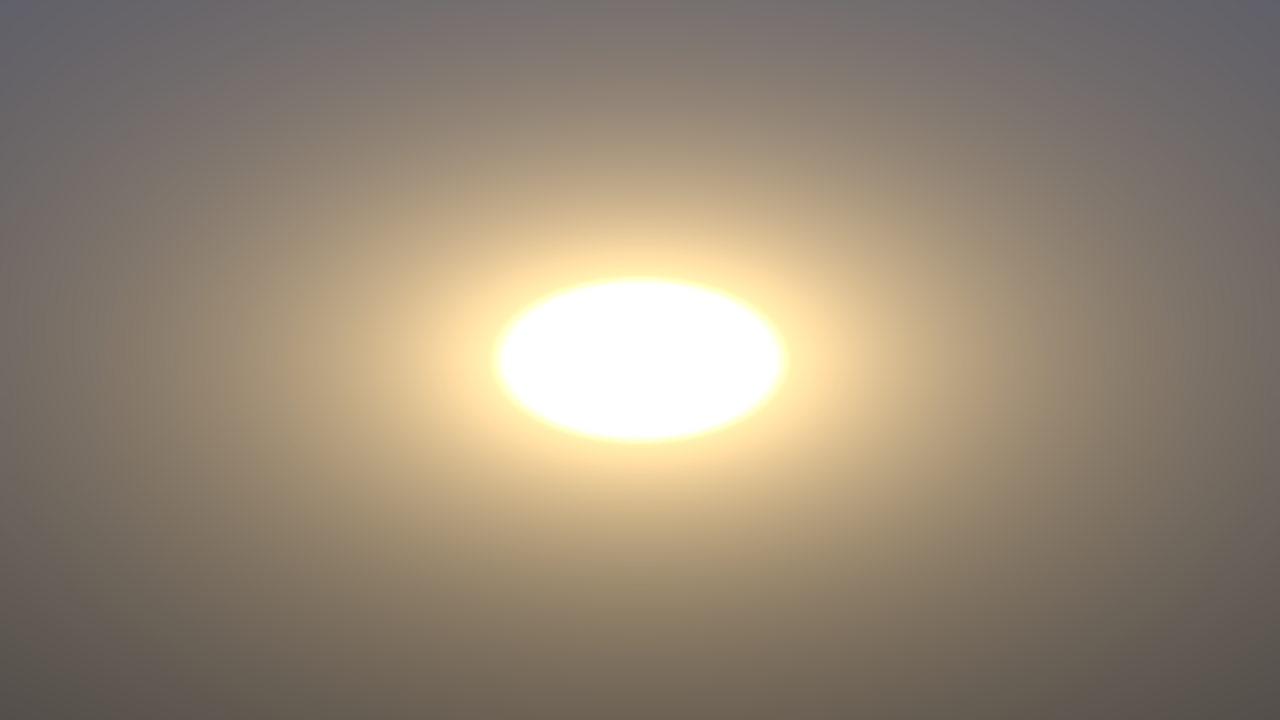
\includegraphics[width=0.82\textwidth]{captura_execucao.png}
    \caption{Captura de tela obtida diretamente do \textit{framebuffer} durante a execução do programa em Vulkan. Demonstra a operação integrada da janela GLFW, \textit{swapchain}, alocação de comandos na GPU e execução dos \textit{shaders} SPIR-V via pipeline gráfico.}
    \label{fig:captura_execucao}
\end{figure}

\subsection{Funcionalidades Concluídas e Próximos Passos}

\textbf{Funcionalidades Implementadas e Validadas nesta Etapa:}
\begin{itemize}
    \setlength{\itemsep}{0pt}
    \item Inicialização completa da instância Vulkan e integração das camadas de validação;
    \item Seleção automática de GPU discreta de alto desempenho e criação do dispositivo lógico;
    \item Identificação e separação das filas gráficas e de apresentação;
    \item Configuração dinâmica e segura da \textit{swapchain} e instanciação das \textit{Image Views};
    \item Criação de \textit{Render Pass}, \textit{Pipeline Layout}, \textit{Framebuffers} e \textit{Pipeline Gráfico};
    \item Alocação de \textit{Command Pool} e múltiplos \textit{Command Buffers};
    \item Sincronização explícita via semáforos de aquisição/renderização e \textit{fences} de CPU-GPU;
    \item Laço principal de aquisição, gravação de comandos, submissão gráfica e apresentação na tela;
    \item Compilação e carga em memória de todos os oito \textit{shaders} SPIR-V projetados;
    \item Desalocação rigorosa e ordenada de todos os recursos da GPU no encerramento da aplicação.
\end{itemize}

\textbf{Funcionalidades para as Próximas Entregas (Técnica de Bloom Completa):}
Nas próximas etapas, o pipeline base construído aqui será expandido para materializar o fluxo completo de onze passes projetado na Entrega 2:
\begin{enumerate}
    \setlength{\itemsep}{0pt}
    \item Alocação dos anexos intermediários fora de tela (\textit{offscreen}) em ponto flutuante de 16 bits (\texttt{VK\_FORMAT\_R16G16B16A16\_SFLOAT}) para a imagem \texttt{sceneHDR};
    \item Criação da textura piramidal de \textit{Bloom} (\texttt{bloomMip[0]} a \texttt{bloomMip[4]});
    \item Configuração dos \textit{Descriptor Sets} e \textit{Uniform Buffers} (\texttt{BloomParams} e \texttt{CameraUBO});
    \item Encadeamento dos passes de \textit{downsample} e \textit{upsample} com mistura aditiva (\textit{additive blending});
    \item Inserção das barreiras de memória explícitas (\texttt{VkImageMemoryBarrier}) entre as etapas de escrita e leitura de texturas.
\end{enumerate}
\fussy

% ===============================================================

\section{Integração do Código e Boilerplate Vulkan}
\label{sec:boilerplate}
\sloppy

Esta seção documenta a quarta entrega do trabalho, cujo objetivo é a construção da infraestrutura básica (\textit{boilerplate}) da aplicação gráfica em C++20 utilizando a API Vulkan, além da integração e validação dos \textit{shaders} desenvolvidos na Entrega 3 (Seção~\ref{sec:pseudocodigo}).

A aplicação desenvolvida abre uma janela interativa, inicializa as estruturas fundamentais do Vulkan, seleciona a GPU do sistema, configura a \textit{swapchain}, aloca os \textit{command buffers}, gerencia primitivas explícitas de sincronização (semáforos e \textit{fences}) e executa o ciclo de renderização na tela. Além disso, todos os oito \textit{shaders} em SPIR-V são carregados em módulos Vulkan (\texttt{VkShaderModule}) e utilizados pelo pipeline gráfico.

\subsection{Organização Modular do Projeto}
Em conformidade com os princípios da responsabilidade única (SOLID) e do código limpo (\textit{clean code}), o projeto foi estruturado em módulos independentes na pasta \texttt{src/}:

\begin{itemize}
    \setlength{\itemsep}{0pt}
    \item \textbf{\texttt{Janela} (\texttt{Janela.hpp/cpp}):} Encapsula a biblioteca GLFW, gerenciando a criação da janela sem contexto OpenGL, redimensionamentos e a criação da superfície \texttt{VkSurfaceKHR}.
    \item \textbf{\texttt{InstanciaVulkan} (\texttt{DispositivoVulkan.hpp/cpp}):} Configura a instância global da API (\texttt{VkInstance}), consulta extensões necessárias e ativa as camadas de validação (\texttt{VK\_LAYER\_KHRONOS\_validation}) com mensagens de depuração (\texttt{VkDebugUtilsMessengerEXT}).
    \item \textbf{\texttt{DispositivoVulkan} (\texttt{DispositivoVulkan.hpp/cpp}):} Identifica as GPUs físicas disponíveis, selecionando preferencialmente dispositivos dedicados (\textit{Discrete GPU}), consulta as famílias de filas com suporte a comandos gráficos e de apresentação, e cria o dispositivo lógico (\texttt{VkDevice}).
    \item \textbf{\texttt{GerenciadorSwapchain} (\texttt{GerenciadorSwapchain.hpp/cpp}):} Negocia com a superfície o melhor formato de cores (preferencialmente \texttt{VK\_FORMAT\_B8G8R8A8\_SRGB}), o modo de apresentação (\textit{Mailbox} para \textit{triple buffering} ou \textit{FIFO}) e a resolução real dos \textit{framebuffers}, instanciando as respectivas \texttt{VkImageView}s. Trata também a recriação automática da cadeia de troca quando a janela é redimensionada.
    \item \textbf{\texttt{CarregadorShader} (\texttt{CarregadorShader.hpp/cpp}):} Lê os arquivos binários compilados em SPIR-V (\texttt{.spv}) do disco e instancia os respectivos módulos Vulkan (\texttt{VkShaderModule}), gerenciando sua validação e destruição controlada.
    \item \textbf{\texttt{PipelineGrafico} (\texttt{PipelineGrafico.hpp/cpp}):} Define o \textit{Render Pass} com transições de layout, cria os \textit{Framebuffers} vinculados às imagens da \textit{swapchain} e monta o pipeline gráfico de rasterização com estágios programáveis e estados dinâmicos (\textit{viewport} e \textit{scissor}).
    \item \textbf{\texttt{AplicacaoVulkan} (\texttt{AplicacaoVulkan.hpp/cpp}):} Orquestra o ciclo de vida completo: cria o \textit{Command Pool}, aloca os \textit{Command Buffers}, inicializa semáforos e cercas (\textit{fences}) para sincronização de múltiplos quadros em voo (\textit{frames in flight}), grava os comandos de desenho e controla o laço principal (\textit{main loop}).
\end{itemize}

\subsection{Compilação dos Shaders para SPIR-V}
Os \textit{shaders} desenvolvidos em sintaxe GLSL na Entrega 3 foram compilados para o formato binário padrão do Vulkan (SPIR-V) por meio do compilador oficial \texttt{glslc}, componente do Vulkan SDK.

Foi criado o script automatizado \texttt{compilar\_shaders.sh}, que percorre todos os arquivos \texttt{.vert} e \texttt{.frag} da pasta \texttt{shaders/} e gera as saídas equivalentes em \texttt{shaders/spv/}. Além disso, o sistema de build \texttt{CMakeLists.txt} integra esse alvo (\texttt{compilar\_shaders}) antes da compilação do executável principal, garantindo que qualquer alteração nos \textit{shaders} seja automaticamente refletida nos binários SPIR-V.

\begin{table}[H]
    \centering
    \caption{\textit{Shaders} SPIR-V integrados e carregados na aplicação Vulkan.}
    \label{tab:shaders_spv}
    \vspace{4pt}
    \small
    \begin{tabular}{l l l p{6.5cm}}
        \toprule
        \textbf{Arquivo Fonte} & \textbf{Binário SPIR-V} & \textbf{Estágio} & \textbf{Papel na Técnica de Bloom} \\
        \midrule
        \texttt{scene.vert} & \texttt{scene.vert.spv} & \textit{Vertex} & Transformação de geometria 3D da cena \\
        \texttt{scene.frag} & \texttt{scene.frag.spv} & \textit{Fragment} & Iluminação direta e saída HDR sem corte \\
        \texttt{fullscreen.vert} & \texttt{fullscreen.vert.spv} & \textit{Vertex} & Geração procedural do triângulo de tela cheia \\
        \texttt{bright.frag} & \texttt{bright.frag.spv} & \textit{Fragment} & Isolamento de altas luzes (\textit{bright pass}) \\
        \texttt{downsample.frag} & \texttt{downsample.frag.spv} & \textit{Fragment} & Redução piramidal e filtro de 13 amostras \\
        \texttt{upsample.frag} & \texttt{upsample.frag.spv} & \textit{Fragment} & Expansão piramidal e filtro tenda $3\times3$ \\
        \texttt{composite.frag} & \texttt{composite.frag.spv} & \textit{Fragment} & Composição da cena com \textit{Bloom} e \textit{Tone Mapping} \\
        \texttt{teste.frag} & \texttt{teste.frag.spv} & \textit{Fragment} & Fragmento de teste visual com gradiente e núcleo luminoso \\
        \bottomrule
    \end{tabular}
\end{table}

\subsection{Ferramentas, Bibliotecas e Ambiente de Execução}
A infraestrutura foi construída e validada no seguinte ambiente técnico:
\begin{itemize}
    \setlength{\itemsep}{0pt}
    \item \textbf{Linguagem e Padrão:} C++20 (ISO/IEC 14882:2020), utilizando recursos como \texttt{std::optional}, ponteiros inteligentes (\texttt{std::unique\_ptr}) e verificação rigorosa de tipos.
    \item \textbf{Compilador:} GNU Compiler Collection (\texttt{g++} 16.2.1 / \texttt{gcc}) com suporte a flags de otimização e checagem estrita de avisos (\texttt{-Wall -Wextra -Wpedantic}).
    \item \textbf{Sistema de Build:} CMake versão 3.20 ou superior.
    \item \textbf{Vulkan SDK / Header:} Vulkan API versão 1.3 / 1.4 (especificação 1.4.364), biblioteca carregadora \texttt{libvulkan.so.1}.
    \item \textbf{Compilador de Shaders:} \texttt{glslc} (Vulkan Shader Compiler via Google Shaderc).
    \item \textbf{Bibliotecas Auxiliares:} GLFW 3.3 (gerenciamento de janelas e contexto de superfície do sistema operacional) e GLM (álgebra linear e estruturas matriciais/vetoriais).
    \item \textbf{GPU de Execução:} NVIDIA GeForce RTX 3080 (driver proprietário versão 615.71, suporte nativo à API Vulkan 1.4).
\end{itemize}

\subsection{Instruções de Compilação e Execução}

Para compilar e executar o projeto no Linux a partir do terminal:

\begin{enumerate}
    \item \textbf{Compilação dos Shaders (opcional, já acoplada ao CMake):}
    \begin{verbatim}
    ./compilar_shaders.sh
    \end{verbatim}
    \item \textbf{Geração dos arquivos de build com CMake:}
    \begin{verbatim}
    cmake -B build
    \end{verbatim}
    \item \textbf{Compilação do executável:}
    \begin{verbatim}
    cmake --build build
    \end{verbatim}
    \item \textbf{Execução da aplicação:}
    \begin{verbatim}
    ./build/BloomVulkan
    \end{verbatim}
    Para testes automatizados sem intervenção de usuário, a aplicação aceita o parâmetro \texttt{--quadros N} (ou \texttt{--teste}), que renderiza $N$ quadros, exporta a comprovação visual e finaliza de forma limpa.
\end{enumerate}

\subsection{Comprovação Visual e Funcionamento}
Ao executar a aplicação, o Vulkan inicializa a superfície de apresentação na janela criada via GLFW e associa o pipeline gráfico aos módulos SPIR-V \texttt{fullscreen.vert.spv} e \texttt{teste.frag.spv}. 

O \texttt{fullscreen.vert} gera dinamicamente as coordenadas do triângulo de tela cheia sem necessidade de \textit{vertex buffer} físico, e o \textit{fragment shader} interpola as coordenadas UV de tela cheia, desenhando um gradiente de luminância e um núcleo emissivo incandescente central. A Figura~\ref{fig:captura_execucao} ilustra a captura de tela direta gerada na renderização da GPU.

\begin{figure}[H]
    \centering
    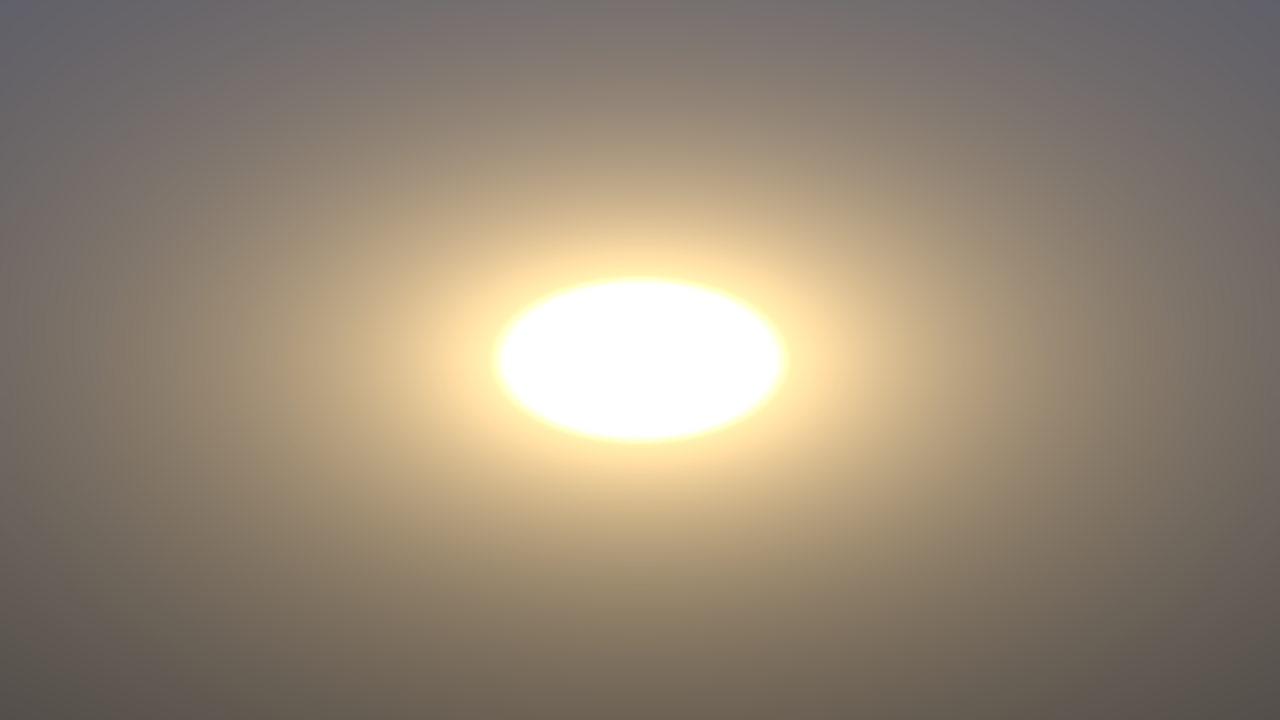
\includegraphics[width=0.82\textwidth]{captura_execucao.png}
    \caption{Captura de tela obtida diretamente do \textit{framebuffer} durante a execução do programa em Vulkan. Demonstra a operação integrada da janela GLFW, \textit{swapchain}, alocação de comandos na GPU e execução dos \textit{shaders} SPIR-V via pipeline gráfico.}
    \label{fig:captura_execucao}
\end{figure}

\subsection{Funcionalidades Concluídas e Próximos Passos}

\textbf{Funcionalidades Implementadas e Validadas nesta Etapa:}
\begin{itemize}
    \setlength{\itemsep}{0pt}
    \item Inicialização completa da instância Vulkan e integração das camadas de validação;
    \item Seleção automática de GPU discreta de alto desempenho e criação do dispositivo lógico;
    \item Identificação e separação das filas gráficas e de apresentação;
    \item Configuração dinâmica e segura da \textit{swapchain} e instanciação das \textit{Image Views};
    \item Criação de \textit{Render Pass}, \textit{Pipeline Layout}, \textit{Framebuffers} e \textit{Pipeline Gráfico};
    \item Alocação de \textit{Command Pool} e múltiplos \textit{Command Buffers};
    \item Sincronização explícita via semáforos de aquisição/renderização e \textit{fences} de CPU-GPU;
    \item Laço principal de aquisição, gravação de comandos, submissão gráfica e apresentação na tela;
    \item Compilação e carga em memória de todos os oito \textit{shaders} SPIR-V projetados;
    \item Desalocação rigorosa e ordenada de todos os recursos da GPU no encerramento da aplicação.
\end{itemize}

\textbf{Funcionalidades para as Próximas Entregas (Técnica de Bloom Completa):}
Nas próximas etapas, o pipeline base construído aqui será expandido para materializar o fluxo completo de onze passes projetado na Entrega 2:
\begin{enumerate}
    \setlength{\itemsep}{0pt}
    \item Alocação dos anexos intermediários fora de tela (\textit{offscreen}) em ponto flutuante de 16 bits (\texttt{VK\_FORMAT\_R16G16B16A16\_SFLOAT}) para a imagem \texttt{sceneHDR};
    \item Criação da textura piramidal de \textit{Bloom} (\texttt{bloomMip[0]} a \texttt{bloomMip[4]});
    \item Configuração dos \textit{Descriptor Sets} e \textit{Uniform Buffers} (\texttt{BloomParams} e \texttt{CameraUBO});
    \item Encadeamento dos passes de \textit{downsample} e \textit{upsample} com mistura aditiva (\textit{additive blending});
    \item Inserção das barreiras de memória explícitas (\texttt{VkImageMemoryBarrier}) entre as etapas de escrita e leitura de texturas.
\end{enumerate}
\fussy

% ===============================================================

\section{Integração do Código e Boilerplate Vulkan}
\label{sec:boilerplate}
\sloppy

Esta seção documenta a quarta entrega do trabalho, cujo objetivo é a construção da infraestrutura básica (\textit{boilerplate}) da aplicação gráfica em C++20 utilizando a API Vulkan, além da integração e validação dos \textit{shaders} desenvolvidos na Entrega 3 (Seção~\ref{sec:pseudocodigo}).

A aplicação desenvolvida abre uma janela interativa, inicializa as estruturas fundamentais do Vulkan, seleciona a GPU do sistema, configura a \textit{swapchain}, aloca os \textit{command buffers}, gerencia primitivas explícitas de sincronização (semáforos e \textit{fences}) e executa o ciclo de renderização na tela. Além disso, todos os oito \textit{shaders} em SPIR-V são carregados em módulos Vulkan (\texttt{VkShaderModule}) e utilizados pelo pipeline gráfico.

\subsection{Organização Modular do Projeto}
Em conformidade com os princípios da responsabilidade única (SOLID) e do código limpo (\textit{clean code}), o projeto foi estruturado em módulos independentes na pasta \texttt{src/}:

\begin{itemize}
    \setlength{\itemsep}{0pt}
    \item \textbf{\texttt{Janela} (\texttt{Janela.hpp/cpp}):} Encapsula a biblioteca GLFW, gerenciando a criação da janela sem contexto OpenGL, redimensionamentos e a criação da superfície \texttt{VkSurfaceKHR}.
    \item \textbf{\texttt{InstanciaVulkan} (\texttt{DispositivoVulkan.hpp/cpp}):} Configura a instância global da API (\texttt{VkInstance}), consulta extensões necessárias e ativa as camadas de validação (\texttt{VK\_LAYER\_KHRONOS\_validation}) com mensagens de depuração (\texttt{VkDebugUtilsMessengerEXT}).
    \item \textbf{\texttt{DispositivoVulkan} (\texttt{DispositivoVulkan.hpp/cpp}):} Identifica as GPUs físicas disponíveis, selecionando preferencialmente dispositivos dedicados (\textit{Discrete GPU}), consulta as famílias de filas com suporte a comandos gráficos e de apresentação, e cria o dispositivo lógico (\texttt{VkDevice}).
    \item \textbf{\texttt{GerenciadorSwapchain} (\texttt{GerenciadorSwapchain.hpp/cpp}):} Negocia com a superfície o melhor formato de cores (preferencialmente \texttt{VK\_FORMAT\_B8G8R8A8\_SRGB}), o modo de apresentação (\textit{Mailbox} para \textit{triple buffering} ou \textit{FIFO}) e a resolução real dos \textit{framebuffers}, instanciando as respectivas \texttt{VkImageView}s. Trata também a recriação automática da cadeia de troca quando a janela é redimensionada.
    \item \textbf{\texttt{CarregadorShader} (\texttt{CarregadorShader.hpp/cpp}):} Lê os arquivos binários compilados em SPIR-V (\texttt{.spv}) do disco e instancia os respectivos módulos Vulkan (\texttt{VkShaderModule}), gerenciando sua validação e destruição controlada.
    \item \textbf{\texttt{PipelineGrafico} (\texttt{PipelineGrafico.hpp/cpp}):} Define o \textit{Render Pass} com transições de layout, cria os \textit{Framebuffers} vinculados às imagens da \textit{swapchain} e monta o pipeline gráfico de rasterização com estágios programáveis e estados dinâmicos (\textit{viewport} e \textit{scissor}).
    \item \textbf{\texttt{AplicacaoVulkan} (\texttt{AplicacaoVulkan.hpp/cpp}):} Orquestra o ciclo de vida completo: cria o \textit{Command Pool}, aloca os \textit{Command Buffers}, inicializa semáforos e cercas (\textit{fences}) para sincronização de múltiplos quadros em voo (\textit{frames in flight}), grava os comandos de desenho e controla o laço principal (\textit{main loop}).
\end{itemize}

\subsection{Compilação dos Shaders para SPIR-V}
Os \textit{shaders} desenvolvidos em sintaxe GLSL na Entrega 3 foram compilados para o formato binário padrão do Vulkan (SPIR-V) por meio do compilador oficial \texttt{glslc}, componente do Vulkan SDK.

Foi criado o script automatizado \texttt{compilar\_shaders.sh}, que percorre todos os arquivos \texttt{.vert} e \texttt{.frag} da pasta \texttt{shaders/} e gera as saídas equivalentes em \texttt{shaders/spv/}. Além disso, o sistema de build \texttt{CMakeLists.txt} integra esse alvo (\texttt{compilar\_shaders}) antes da compilação do executável principal, garantindo que qualquer alteração nos \textit{shaders} seja automaticamente refletida nos binários SPIR-V.

\begin{table}[H]
    \centering
    \caption{\textit{Shaders} SPIR-V integrados e carregados na aplicação Vulkan.}
    \label{tab:shaders_spv}
    \vspace{4pt}
    \small
    \begin{tabular}{l l l p{6.5cm}}
        \toprule
        \textbf{Arquivo Fonte} & \textbf{Binário SPIR-V} & \textbf{Estágio} & \textbf{Papel na Técnica de Bloom} \\
        \midrule
        \texttt{scene.vert} & \texttt{scene.vert.spv} & \textit{Vertex} & Transformação de geometria 3D da cena \\
        \texttt{scene.frag} & \texttt{scene.frag.spv} & \textit{Fragment} & Iluminação direta e saída HDR sem corte \\
        \texttt{fullscreen.vert} & \texttt{fullscreen.vert.spv} & \textit{Vertex} & Geração procedural do triângulo de tela cheia \\
        \texttt{bright.frag} & \texttt{bright.frag.spv} & \textit{Fragment} & Isolamento de altas luzes (\textit{bright pass}) \\
        \texttt{downsample.frag} & \texttt{downsample.frag.spv} & \textit{Fragment} & Redução piramidal e filtro de 13 amostras \\
        \texttt{upsample.frag} & \texttt{upsample.frag.spv} & \textit{Fragment} & Expansão piramidal e filtro tenda $3\times3$ \\
        \texttt{composite.frag} & \texttt{composite.frag.spv} & \textit{Fragment} & Composição da cena com \textit{Bloom} e \textit{Tone Mapping} \\
        \texttt{teste.frag} & \texttt{teste.frag.spv} & \textit{Fragment} & Fragmento de teste visual com gradiente e núcleo luminoso \\
        \bottomrule
    \end{tabular}
\end{table}

\subsection{Ferramentas, Bibliotecas e Ambiente de Execução}
A infraestrutura foi construída e validada no seguinte ambiente técnico:
\begin{itemize}
    \setlength{\itemsep}{0pt}
    \item \textbf{Linguagem e Padrão:} C++20 (ISO/IEC 14882:2020), utilizando recursos como \texttt{std::optional}, ponteiros inteligentes (\texttt{std::unique\_ptr}) e verificação rigorosa de tipos.
    \item \textbf{Compilador:} GNU Compiler Collection (\texttt{g++} 16.2.1 / \texttt{gcc}) com suporte a flags de otimização e checagem estrita de avisos (\texttt{-Wall -Wextra -Wpedantic}).
    \item \textbf{Sistema de Build:} CMake versão 3.20 ou superior.
    \item \textbf{Vulkan SDK / Header:} Vulkan API versão 1.3 / 1.4 (especificação 1.4.364), biblioteca carregadora \texttt{libvulkan.so.1}.
    \item \textbf{Compilador de Shaders:} \texttt{glslc} (Vulkan Shader Compiler via Google Shaderc).
    \item \textbf{Bibliotecas Auxiliares:} GLFW 3.3 (gerenciamento de janelas e contexto de superfície do sistema operacional) e GLM (álgebra linear e estruturas matriciais/vetoriais).
    \item \textbf{GPU de Execução:} NVIDIA GeForce RTX 3080 (driver proprietário versão 615.71, suporte nativo à API Vulkan 1.4).
\end{itemize}

\subsection{Instruções de Compilação e Execução}

Para compilar e executar o projeto no Linux a partir do terminal:

\begin{enumerate}
    \item \textbf{Compilação dos Shaders (opcional, já acoplada ao CMake):}
    \begin{verbatim}
    ./compilar_shaders.sh
    \end{verbatim}
    \item \textbf{Geração dos arquivos de build com CMake:}
    \begin{verbatim}
    cmake -B build
    \end{verbatim}
    \item \textbf{Compilação do executável:}
    \begin{verbatim}
    cmake --build build
    \end{verbatim}
    \item \textbf{Execução da aplicação:}
    \begin{verbatim}
    ./build/BloomVulkan
    \end{verbatim}
    Para testes automatizados sem intervenção de usuário, a aplicação aceita o parâmetro \texttt{--quadros N} (ou \texttt{--teste}), que renderiza $N$ quadros, exporta a comprovação visual e finaliza de forma limpa.
\end{enumerate}

\subsection{Comprovação Visual e Funcionamento}
Ao executar a aplicação, o Vulkan inicializa a superfície de apresentação na janela criada via GLFW e associa o pipeline gráfico aos módulos SPIR-V \texttt{fullscreen.vert.spv} e \texttt{teste.frag.spv}. 

O \texttt{fullscreen.vert} gera dinamicamente as coordenadas do triângulo de tela cheia sem necessidade de \textit{vertex buffer} físico, e o \textit{fragment shader} interpola as coordenadas UV de tela cheia, desenhando um gradiente de luminância e um núcleo emissivo incandescente central. A Figura~\ref{fig:captura_execucao} ilustra a captura de tela direta gerada na renderização da GPU.

\begin{figure}[H]
    \centering
    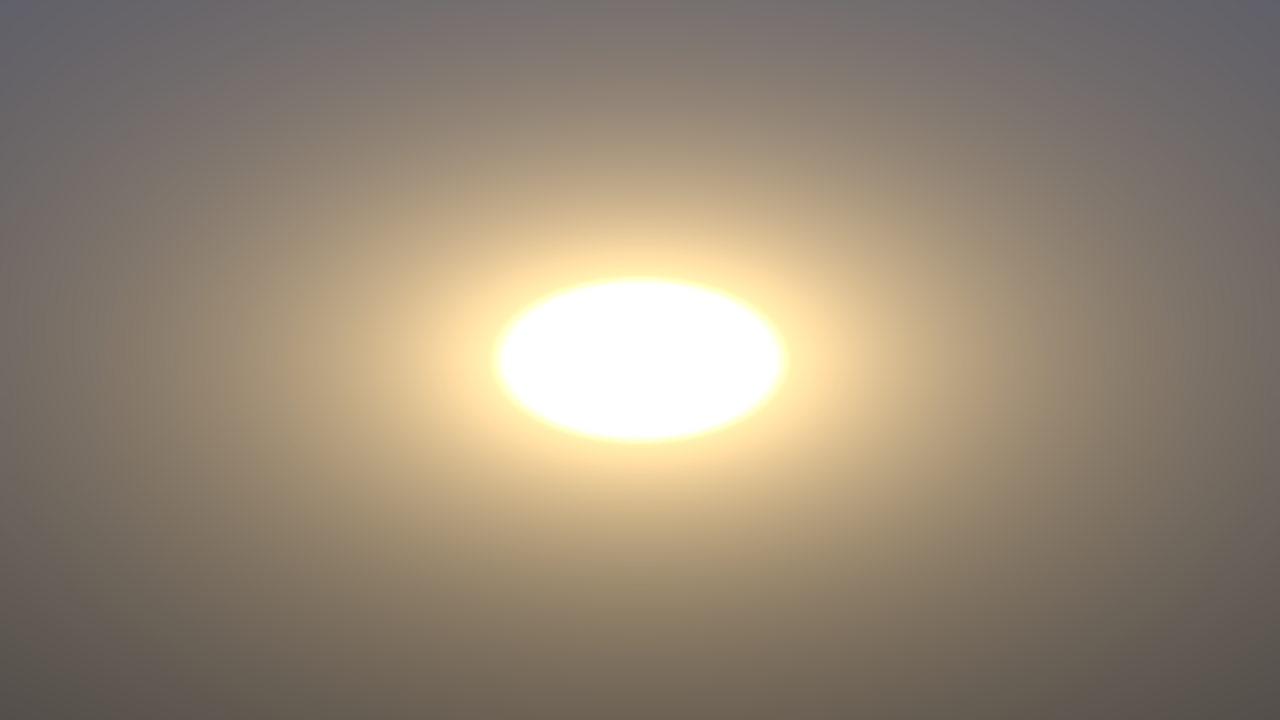
\includegraphics[width=0.82\textwidth]{captura_execucao.png}
    \caption{Captura de tela obtida diretamente do \textit{framebuffer} durante a execução do programa em Vulkan. Demonstra a operação integrada da janela GLFW, \textit{swapchain}, alocação de comandos na GPU e execução dos \textit{shaders} SPIR-V via pipeline gráfico.}
    \label{fig:captura_execucao}
\end{figure}

\subsection{Funcionalidades Concluídas e Próximos Passos}

\textbf{Funcionalidades Implementadas e Validadas nesta Etapa:}
\begin{itemize}
    \setlength{\itemsep}{0pt}
    \item Inicialização completa da instância Vulkan e integração das camadas de validação;
    \item Seleção automática de GPU discreta de alto desempenho e criação do dispositivo lógico;
    \item Identificação e separação das filas gráficas e de apresentação;
    \item Configuração dinâmica e segura da \textit{swapchain} e instanciação das \textit{Image Views};
    \item Criação de \textit{Render Pass}, \textit{Pipeline Layout}, \textit{Framebuffers} e \textit{Pipeline Gráfico};
    \item Alocação de \textit{Command Pool} e múltiplos \textit{Command Buffers};
    \item Sincronização explícita via semáforos de aquisição/renderização e \textit{fences} de CPU-GPU;
    \item Laço principal de aquisição, gravação de comandos, submissão gráfica e apresentação na tela;
    \item Compilação e carga em memória de todos os oito \textit{shaders} SPIR-V projetados;
    \item Desalocação rigorosa e ordenada de todos os recursos da GPU no encerramento da aplicação.
\end{itemize}

\textbf{Funcionalidades para as Próximas Entregas (Técnica de Bloom Completa):}
Nas próximas etapas, o pipeline base construído aqui será expandido para materializar o fluxo completo de onze passes projetado na Entrega 2:
\begin{enumerate}
    \setlength{\itemsep}{0pt}
    \item Alocação dos anexos intermediários fora de tela (\textit{offscreen}) em ponto flutuante de 16 bits (\texttt{VK\_FORMAT\_R16G16B16A16\_SFLOAT}) para a imagem \texttt{sceneHDR};
    \item Criação da textura piramidal de \textit{Bloom} (\texttt{bloomMip[0]} a \texttt{bloomMip[4]});
    \item Configuração dos \textit{Descriptor Sets} e \textit{Uniform Buffers} (\texttt{BloomParams} e \texttt{CameraUBO});
    \item Encadeamento dos passes de \textit{downsample} e \textit{upsample} com mistura aditiva (\textit{additive blending});
    \item Inserção das barreiras de memória explícitas (\texttt{VkImageMemoryBarrier}) entre as etapas de escrita e leitura de texturas.
\end{enumerate}
\fussy
